\section{Outlier-Detection Methods}

\begin{frame}{How can we detect outliers?}
	\begin{itemize}
		\item \textbf{Two ways to categorize outlier-detection methods:}
		      \begin{itemize}
			      \item Based on whether \textbf{\color{airforceblue}user-labeled examples of outliers} can be obtained: \\
			            I.e. supervised, semi-supervised vs. unsupervised methods.
			      \item Based on \textbf{\color{airforceblue}assumptions} about normal data and outliers: \\
			            I.e. statistical, proximity-based, and clustering-based methods.
		      \end{itemize}
	\end{itemize}
\end{frame}


\begin{frame}{Outlier Detection I}
	\begin{itemize}
		\item \textbf{Supervised Methods:}
		      \begin{itemize}
			      \item Modeling outlier detection as a \textbf{classification problem}:\\
			            Samples examined by domain experts used for training \& testing.
			      \item Methods for learning a classifier for outlier detection effectively:
			            \begin{itemize}
				            \item Model normal objects \& report those not matching the model as outliers.
				            \item Model outliers and treat those not matching the model as normal.
			            \end{itemize}
			      \item \textbf{Challenges:}
			            \begin{itemize}
				            \item Imbalanced classes, i.e., outliers are rare: \\
				                  Boost the outlier class and make up some artificial outliers.
				            \item Catch as many outliers as possible, \\
				                  i.e., recall is more important than accuracy \\
				                  (i.e., not mislabeling normal objects as outliers).
			            \end{itemize}
		      \end{itemize}
	\end{itemize}
\end{frame}


\begin{frame}
	\frametitle{Outlier Detection II}
	\begin{itemize}
		\item \textbf{Assume the {\color{airforceblue}normal objects are somewhat "clustered"} into multiple groups, each having some distinct features.}
		      \item\textbf{An outlier is expected to be {\color{airforceblue}far away from any group} of normal objects.}
		\item \textbf{Weakness: Can't detect collective outliers effectively.}
		      \begin{itemize}
			      \item Normal objects may not share any strong pattern, \\
			            but the collective outliers may have high similarity in a small area.
		      \end{itemize}
		\item \textbf{I.e., in some intrusion or virus detection, normal activities are diverse.}
		      \begin{itemize}
			      \item Unsupervised methods may have a high false-positive rate, \\
			            but still miss many real outliers.
			      \item Supervised methods can be more effective, \\
			            e.g., identify attacking some key resources.
		      \end{itemize}
	\end{itemize}
\end{frame}


\begin{frame}
	\frametitle{Outlier Detection III}
	\begin{itemize}
		\item \textbf{Many clustering methods can be adapted for unsupervised methods:}
		      \begin{itemize}
			      \item Find clusters, then outliers: not belonging to any cluster.
			      \item \textbf{Problem 1:} Hard to distinguish noise from outliers.
			      \item \textbf{Problem 2:} Costly since first clustering, but far less outliers than normal objects.
			      \item Newer methods: tackle outliers directly.
		      \end{itemize}
	\end{itemize}
\end{frame}


\begin{frame}
	\frametitle{Outlier Detection IV}
	\begin{itemize}
		\item \textbf{Situation:}
		      \begin{itemize}
			      \item In many applications, the \textbf{\color{airforceblue}number of labeled data objects is small}:\\
			            Labels could be on outliers only, on normal objects only, or on both.
		      \end{itemize}
		\item \textbf{Semi-supervised outlier detection:}
		      \begin{itemize}
			      \item Regarded as application of semi-supervised learning.
		      \end{itemize}
		\item \textbf{If some {\color{airforceblue}labeled normal objects} are available:}
		      \begin{itemize}
			      \item Use the labeled examples and the proximate \\
			            unlabeled objects to train a model for normal objects.
			      \item Those not fitting the model of normal objects are detected as outliers.
		      \end{itemize}
		\item \textbf{If only some {\color{airforceblue}labeled outliers} are available, \\ that small number may not cover the possible outliers well.}
		      \begin{itemize}
			      \item To improve the quality of outlier detection: get help from models for normal objects learned from unsupervised methods.
		      \end{itemize}
	\end{itemize}
\end{frame}


\begin{frame}{Outlier Detection V: Statistical Methods}
	\tikzoverlay at (11cm,1cm) {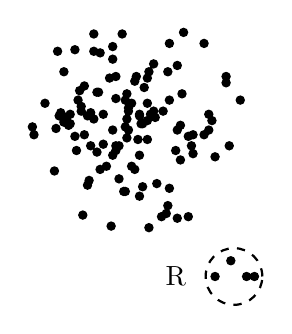
\begin{tikzpicture}[thick,scale=2, every node/.style={scale=5}]
	\fill (1.21, 0.56)  circle (0.3mm) (0.51, 1.02)  circle (0.3mm) (0.61, 1.44)  circle (0.3mm) (0.91, 1.54)  circle (0.3mm) (0.69, 0.58)  circle (0.3mm) (1.2, 1.3)  circle (0.3mm) (1.28, 0.96)  circle (0.3mm) (0.67, 1.21)  circle (0.3mm) (0.34, 0.95)  circle (0.3mm) (0.89, 0.83)  circle (0.3mm) (1.33, 0.38)  circle (0.3mm) (1.3, 1.55)  circle (0.3mm) (1.07, 0.99)  circle (0.3mm) (0.89, 0.62)  circle (0.3mm) (1.07, 0.87)  circle (0.3mm) (0.48, 0.67)  circle (0.3mm) (0.35, 0.9)  circle (0.3mm) (1.26, 1.34)  circle (0.3mm) (0.73, 1.54)  circle (0.3mm) (0.76, 1.17)  circle (0.3mm) (1.02, 1.03)  circle (0.3mm) (1.28, 0.74)  circle (0.3mm) (0.54, 1.3)  circle (0.3mm) (0.73, 1.43)  circle (0.3mm) (0.77, 1.42)  circle (0.3mm) (0.85, 0.93)  circle (0.3mm) (0.97, 1.1)  circle (0.3mm) (1.08, 1.3)  circle (0.3mm) (0.5, 1.43)  circle (0.3mm) (1.25, 0.8)  circle (0.3mm) (1.59, 0.83)  circle (0.3mm) (1.02, 0.51)  circle (0.3mm) (0.79, 0.84)  circle (0.3mm) (1.11, 1.05)  circle (0.3mm) (1.2, 0.45)  circle (0.3mm) (1.66, 1.12)  circle (0.3mm) (0.66, 0.39)  circle (0.3mm) (1.57, 1.27)  circle (0.3mm) (1.19, 0.4)  circle (0.3mm) (0.84, 0.32)  circle (0.3mm) (1.36, 0.9)  circle (0.3mm) (1.21, 1.48)  circle (0.3mm) (1.04, 0.57)  circle (0.3mm) (0.87, 0.83)  circle (0.3mm) (0.92, 0.54)  circle (0.3mm) (0.85, 1.46)  circle (0.3mm) (1.16, 0.38)  circle (0.3mm) (0.94, 0.88)  circle (0.3mm) (1.13, 0.59)  circle (0.3mm) (0.71, 0.83)  circle (0.3mm) (1.26, 0.37)  circle (0.3mm) (1.07, 0.87)  circle (0.3mm) (1.57, 1.23)  circle (0.3mm) (0.62, 0.8)  circle (0.3mm) (1.5, 0.76)  circle (0.3mm) (0.42, 1.1)  circle (0.3mm) (1.43, 1.48)  circle (0.3mm) (1.43, 0.9)  circle (0.3mm) (0.49, 0.94)  circle (0.3mm) (1.08, 0.31)  circle (0.3mm)

	(1.04, 0.97)  circle (0.3mm) (0.95, 0.93)  circle (0.3mm) (1.05, 1.2)  circle (0.3mm) (0.54, 0.98)  circle (0.3mm) (0.71, 1.04)  circle (0.3mm) (0.75, 1.17)  circle (0.3mm) (1.07, 1.26)  circle (0.3mm) (0.63, 1.12)  circle (0.3mm) (0.65, 1.08)  circle (0.3mm) (0.95, 1.05)  circle (0.3mm) (0.83, 1.26)  circle (0.3mm) (0.77, 0.68)  circle (0.3mm) (1.02, 0.77)  circle (0.3mm) (0.64, 1.18)  circle (0.3mm) (0.99, 0.68)  circle (0.3mm) (1.21, 1.12)  circle (0.3mm) (0.75, 0.79)  circle (0.3mm) (1.17, 1.05)  circle (0.3mm) (1.01, 0.87)  circle (0.3mm) (0.69, 1.02)  circle (0.3mm) (1.46, 0.93)  circle (0.3mm) (1.02, 1.02)  circle (0.3mm) (1.26, 0.93)  circle (0.3mm) (1.12, 1.01)  circle (0.3mm) (1.46, 1.03)  circle (0.3mm) (0.93, 0.95)  circle (0.3mm) (0.67, 0.9)  circle (0.3mm) (1.0, 1.27)  circle (0.3mm) (0.99, 1.24)  circle (0.3mm) (0.81, 0.7)  circle (0.3mm) (0.93, 0.54)  circle (0.3mm) (0.97, 0.7)  circle (0.3mm) (0.57, 0.96)  circle (0.3mm) (0.55, 1.01)  circle (0.3mm) (1.33, 0.89)  circle (0.3mm) (0.87, 0.8)  circle (0.3mm) (1.11, 1.35)  circle (0.3mm) (0.85, 1.38)  circle (0.3mm) (0.52, 1.04)  circle (0.3mm) (0.7, 0.61)  circle (0.3mm) (1.48, 0.99)  circle (0.3mm) (1.03, 0.97)  circle (0.3mm) (1.07, 1.1)  circle (0.3mm) (0.65, 1.05)  circle (0.3mm) (0.73, 1.0)  circle (0.3mm) (0.87, 1.13)  circle (0.3mm) (0.87, 1.27)  circle (0.3mm) (1.29, 1.16)  circle (0.3mm) (0.79, 1.03)  circle (0.3mm) (0.94, 1.0)  circle (0.3mm) (0.61, 0.89)  circle (0.3mm) (1.35, 0.83)  circle (0.3mm) (1.36, 0.78)  circle (0.3mm) (0.94, 1.16)  circle (0.3mm) (1.09, 1.03)  circle (0.3mm) (0.85, 0.77)  circle (0.3mm) (0.58, 1.03)  circle (0.3mm) (0.95, 1.07)  circle (0.3mm) (0.58, 0.97)  circle (0.3mm) (0.93, 1.12)  circle (0.3mm);

	\draw[dashed] (1.62,0) circle (1.8mm);
	\fill (1.7,0)  circle (0.3mm) (1.75,0)  circle (0.3mm) (1.5,0)  circle (0.3mm) (1.6,0.1)  circle (0.3mm);
	\node[scale = 0.2] at (1.25,0)    {R};

\end{tikzpicture}
};
	\begin{itemize}
		\item (Also known as model-based methods)
		\item Assume that the \textbf{\color{airforceblue}normal data follow some statistical model}.
		      \begin{itemize}
			      \item The data not following the model are outliers.
		      \end{itemize}
		\item \textbf{Example (right figure):}
		      \begin{itemize}
			      \item First use Gaussian distribution $\mathcal{N}_D(x \; \vert \; \mu,\sigma)$ to model the normal data.
			      \item For each object $y$ in region $R$, estimate $\mathcal{N}_D(y \; \vert \; \mu, \sigma)$, the probability that $y$ \\
			            fits the Gaussian distribution.
			      \item If $\mathcal{N}_D(y \; \vert \; \mu, \sigma)$ is very low, $y$ is unlikely generated by the Gaussian model, thus an outlier.
		      \end{itemize}
		      \item\textbf{Effectiveness of statistical methods:}
		      \begin{itemize}
			      \item Highly depends on whether the assumption of statistical model holds in the real data.
		      \end{itemize}
		\item \textbf{There are many kinds of statistical models.}
		      \begin{itemize}
			      \item E.g., parametric vs. non-parametric.
		      \end{itemize}
	\end{itemize}
\end{frame}


\begin{frame}{Outlier Detection (2): Proximity-Based Methods}
	\tikzoverlay at (11cm,1cm) {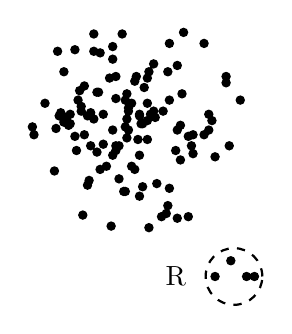
\begin{tikzpicture}[thick,scale=2, every node/.style={scale=5}]
	\fill (1.21, 0.56)  circle (0.3mm) (0.51, 1.02)  circle (0.3mm) (0.61, 1.44)  circle (0.3mm) (0.91, 1.54)  circle (0.3mm) (0.69, 0.58)  circle (0.3mm) (1.2, 1.3)  circle (0.3mm) (1.28, 0.96)  circle (0.3mm) (0.67, 1.21)  circle (0.3mm) (0.34, 0.95)  circle (0.3mm) (0.89, 0.83)  circle (0.3mm) (1.33, 0.38)  circle (0.3mm) (1.3, 1.55)  circle (0.3mm) (1.07, 0.99)  circle (0.3mm) (0.89, 0.62)  circle (0.3mm) (1.07, 0.87)  circle (0.3mm) (0.48, 0.67)  circle (0.3mm) (0.35, 0.9)  circle (0.3mm) (1.26, 1.34)  circle (0.3mm) (0.73, 1.54)  circle (0.3mm) (0.76, 1.17)  circle (0.3mm) (1.02, 1.03)  circle (0.3mm) (1.28, 0.74)  circle (0.3mm) (0.54, 1.3)  circle (0.3mm) (0.73, 1.43)  circle (0.3mm) (0.77, 1.42)  circle (0.3mm) (0.85, 0.93)  circle (0.3mm) (0.97, 1.1)  circle (0.3mm) (1.08, 1.3)  circle (0.3mm) (0.5, 1.43)  circle (0.3mm) (1.25, 0.8)  circle (0.3mm) (1.59, 0.83)  circle (0.3mm) (1.02, 0.51)  circle (0.3mm) (0.79, 0.84)  circle (0.3mm) (1.11, 1.05)  circle (0.3mm) (1.2, 0.45)  circle (0.3mm) (1.66, 1.12)  circle (0.3mm) (0.66, 0.39)  circle (0.3mm) (1.57, 1.27)  circle (0.3mm) (1.19, 0.4)  circle (0.3mm) (0.84, 0.32)  circle (0.3mm) (1.36, 0.9)  circle (0.3mm) (1.21, 1.48)  circle (0.3mm) (1.04, 0.57)  circle (0.3mm) (0.87, 0.83)  circle (0.3mm) (0.92, 0.54)  circle (0.3mm) (0.85, 1.46)  circle (0.3mm) (1.16, 0.38)  circle (0.3mm) (0.94, 0.88)  circle (0.3mm) (1.13, 0.59)  circle (0.3mm) (0.71, 0.83)  circle (0.3mm) (1.26, 0.37)  circle (0.3mm) (1.07, 0.87)  circle (0.3mm) (1.57, 1.23)  circle (0.3mm) (0.62, 0.8)  circle (0.3mm) (1.5, 0.76)  circle (0.3mm) (0.42, 1.1)  circle (0.3mm) (1.43, 1.48)  circle (0.3mm) (1.43, 0.9)  circle (0.3mm) (0.49, 0.94)  circle (0.3mm) (1.08, 0.31)  circle (0.3mm)

	(1.04, 0.97)  circle (0.3mm) (0.95, 0.93)  circle (0.3mm) (1.05, 1.2)  circle (0.3mm) (0.54, 0.98)  circle (0.3mm) (0.71, 1.04)  circle (0.3mm) (0.75, 1.17)  circle (0.3mm) (1.07, 1.26)  circle (0.3mm) (0.63, 1.12)  circle (0.3mm) (0.65, 1.08)  circle (0.3mm) (0.95, 1.05)  circle (0.3mm) (0.83, 1.26)  circle (0.3mm) (0.77, 0.68)  circle (0.3mm) (1.02, 0.77)  circle (0.3mm) (0.64, 1.18)  circle (0.3mm) (0.99, 0.68)  circle (0.3mm) (1.21, 1.12)  circle (0.3mm) (0.75, 0.79)  circle (0.3mm) (1.17, 1.05)  circle (0.3mm) (1.01, 0.87)  circle (0.3mm) (0.69, 1.02)  circle (0.3mm) (1.46, 0.93)  circle (0.3mm) (1.02, 1.02)  circle (0.3mm) (1.26, 0.93)  circle (0.3mm) (1.12, 1.01)  circle (0.3mm) (1.46, 1.03)  circle (0.3mm) (0.93, 0.95)  circle (0.3mm) (0.67, 0.9)  circle (0.3mm) (1.0, 1.27)  circle (0.3mm) (0.99, 1.24)  circle (0.3mm) (0.81, 0.7)  circle (0.3mm) (0.93, 0.54)  circle (0.3mm) (0.97, 0.7)  circle (0.3mm) (0.57, 0.96)  circle (0.3mm) (0.55, 1.01)  circle (0.3mm) (1.33, 0.89)  circle (0.3mm) (0.87, 0.8)  circle (0.3mm) (1.11, 1.35)  circle (0.3mm) (0.85, 1.38)  circle (0.3mm) (0.52, 1.04)  circle (0.3mm) (0.7, 0.61)  circle (0.3mm) (1.48, 0.99)  circle (0.3mm) (1.03, 0.97)  circle (0.3mm) (1.07, 1.1)  circle (0.3mm) (0.65, 1.05)  circle (0.3mm) (0.73, 1.0)  circle (0.3mm) (0.87, 1.13)  circle (0.3mm) (0.87, 1.27)  circle (0.3mm) (1.29, 1.16)  circle (0.3mm) (0.79, 1.03)  circle (0.3mm) (0.94, 1.0)  circle (0.3mm) (0.61, 0.89)  circle (0.3mm) (1.35, 0.83)  circle (0.3mm) (1.36, 0.78)  circle (0.3mm) (0.94, 1.16)  circle (0.3mm) (1.09, 1.03)  circle (0.3mm) (0.85, 0.77)  circle (0.3mm) (0.58, 1.03)  circle (0.3mm) (0.95, 1.07)  circle (0.3mm) (0.58, 0.97)  circle (0.3mm) (0.93, 1.12)  circle (0.3mm);

	\draw[dashed] (1.62,0) circle (1.8mm);
	\fill (1.7,0)  circle (0.3mm) (1.75,0)  circle (0.3mm) (1.5,0)  circle (0.3mm) (1.6,0.1)  circle (0.3mm);
	\node[scale = 0.2] at (1.25,0)    {R};

\end{tikzpicture}
};
	An object is an outlier if the \textbf{\color{airforceblue}nearest neighbors of the object are far away},\\ i.e., the proximity of the object significantly deviates from the proximity\\ of most of the other objects in the same data set.
	\begin{itemize}

		\item \textbf{Example (right figure):}
		      \begin{itemize}
			      \item Model the proximity of an object using its 3 nearest neighbors.
			      \item Objects in region R are substantially different from other objects in the data set.
			      \item Thus the objects in R are outliers.
		      \end{itemize}
		\item \textbf{Effectiveness of proximity-based methods:}
		      \begin{itemize}
			      \item Highly relies on the proximity measure.
			      \item In some applications, proximity or distance measures cannot be obtained easily.
			      \item Often have a difficulty in finding a group of outliers which are close to each other.
		      \end{itemize}
		\item \textbf{Two major types of proximity-based outlier detection:}
		      \begin{itemize}
			      \item Distance-based vs. density-based.
		      \end{itemize}
	\end{itemize}
\end{frame}


\begin{frame}{Outlier Detection (3): Clustering-Based Methods}
	\tikzoverlay at (11cm,1cm) {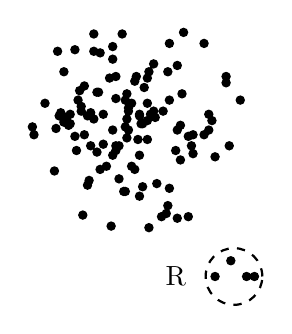
\begin{tikzpicture}[thick,scale=2, every node/.style={scale=5}]
	\fill (1.21, 0.56)  circle (0.3mm) (0.51, 1.02)  circle (0.3mm) (0.61, 1.44)  circle (0.3mm) (0.91, 1.54)  circle (0.3mm) (0.69, 0.58)  circle (0.3mm) (1.2, 1.3)  circle (0.3mm) (1.28, 0.96)  circle (0.3mm) (0.67, 1.21)  circle (0.3mm) (0.34, 0.95)  circle (0.3mm) (0.89, 0.83)  circle (0.3mm) (1.33, 0.38)  circle (0.3mm) (1.3, 1.55)  circle (0.3mm) (1.07, 0.99)  circle (0.3mm) (0.89, 0.62)  circle (0.3mm) (1.07, 0.87)  circle (0.3mm) (0.48, 0.67)  circle (0.3mm) (0.35, 0.9)  circle (0.3mm) (1.26, 1.34)  circle (0.3mm) (0.73, 1.54)  circle (0.3mm) (0.76, 1.17)  circle (0.3mm) (1.02, 1.03)  circle (0.3mm) (1.28, 0.74)  circle (0.3mm) (0.54, 1.3)  circle (0.3mm) (0.73, 1.43)  circle (0.3mm) (0.77, 1.42)  circle (0.3mm) (0.85, 0.93)  circle (0.3mm) (0.97, 1.1)  circle (0.3mm) (1.08, 1.3)  circle (0.3mm) (0.5, 1.43)  circle (0.3mm) (1.25, 0.8)  circle (0.3mm) (1.59, 0.83)  circle (0.3mm) (1.02, 0.51)  circle (0.3mm) (0.79, 0.84)  circle (0.3mm) (1.11, 1.05)  circle (0.3mm) (1.2, 0.45)  circle (0.3mm) (1.66, 1.12)  circle (0.3mm) (0.66, 0.39)  circle (0.3mm) (1.57, 1.27)  circle (0.3mm) (1.19, 0.4)  circle (0.3mm) (0.84, 0.32)  circle (0.3mm) (1.36, 0.9)  circle (0.3mm) (1.21, 1.48)  circle (0.3mm) (1.04, 0.57)  circle (0.3mm) (0.87, 0.83)  circle (0.3mm) (0.92, 0.54)  circle (0.3mm) (0.85, 1.46)  circle (0.3mm) (1.16, 0.38)  circle (0.3mm) (0.94, 0.88)  circle (0.3mm) (1.13, 0.59)  circle (0.3mm) (0.71, 0.83)  circle (0.3mm) (1.26, 0.37)  circle (0.3mm) (1.07, 0.87)  circle (0.3mm) (1.57, 1.23)  circle (0.3mm) (0.62, 0.8)  circle (0.3mm) (1.5, 0.76)  circle (0.3mm) (0.42, 1.1)  circle (0.3mm) (1.43, 1.48)  circle (0.3mm) (1.43, 0.9)  circle (0.3mm) (0.49, 0.94)  circle (0.3mm) (1.08, 0.31)  circle (0.3mm)

	(1.04, 0.97)  circle (0.3mm) (0.95, 0.93)  circle (0.3mm) (1.05, 1.2)  circle (0.3mm) (0.54, 0.98)  circle (0.3mm) (0.71, 1.04)  circle (0.3mm) (0.75, 1.17)  circle (0.3mm) (1.07, 1.26)  circle (0.3mm) (0.63, 1.12)  circle (0.3mm) (0.65, 1.08)  circle (0.3mm) (0.95, 1.05)  circle (0.3mm) (0.83, 1.26)  circle (0.3mm) (0.77, 0.68)  circle (0.3mm) (1.02, 0.77)  circle (0.3mm) (0.64, 1.18)  circle (0.3mm) (0.99, 0.68)  circle (0.3mm) (1.21, 1.12)  circle (0.3mm) (0.75, 0.79)  circle (0.3mm) (1.17, 1.05)  circle (0.3mm) (1.01, 0.87)  circle (0.3mm) (0.69, 1.02)  circle (0.3mm) (1.46, 0.93)  circle (0.3mm) (1.02, 1.02)  circle (0.3mm) (1.26, 0.93)  circle (0.3mm) (1.12, 1.01)  circle (0.3mm) (1.46, 1.03)  circle (0.3mm) (0.93, 0.95)  circle (0.3mm) (0.67, 0.9)  circle (0.3mm) (1.0, 1.27)  circle (0.3mm) (0.99, 1.24)  circle (0.3mm) (0.81, 0.7)  circle (0.3mm) (0.93, 0.54)  circle (0.3mm) (0.97, 0.7)  circle (0.3mm) (0.57, 0.96)  circle (0.3mm) (0.55, 1.01)  circle (0.3mm) (1.33, 0.89)  circle (0.3mm) (0.87, 0.8)  circle (0.3mm) (1.11, 1.35)  circle (0.3mm) (0.85, 1.38)  circle (0.3mm) (0.52, 1.04)  circle (0.3mm) (0.7, 0.61)  circle (0.3mm) (1.48, 0.99)  circle (0.3mm) (1.03, 0.97)  circle (0.3mm) (1.07, 1.1)  circle (0.3mm) (0.65, 1.05)  circle (0.3mm) (0.73, 1.0)  circle (0.3mm) (0.87, 1.13)  circle (0.3mm) (0.87, 1.27)  circle (0.3mm) (1.29, 1.16)  circle (0.3mm) (0.79, 1.03)  circle (0.3mm) (0.94, 1.0)  circle (0.3mm) (0.61, 0.89)  circle (0.3mm) (1.35, 0.83)  circle (0.3mm) (1.36, 0.78)  circle (0.3mm) (0.94, 1.16)  circle (0.3mm) (1.09, 1.03)  circle (0.3mm) (0.85, 0.77)  circle (0.3mm) (0.58, 1.03)  circle (0.3mm) (0.95, 1.07)  circle (0.3mm) (0.58, 0.97)  circle (0.3mm) (0.93, 1.12)  circle (0.3mm);

	\draw[dashed] (1.62,0) circle (1.8mm);
	\fill (1.7,0)  circle (0.3mm) (1.75,0)  circle (0.3mm) (1.5,0)  circle (0.3mm) (1.6,0.1)  circle (0.3mm);
	\node[scale = 0.2] at (1.25,0)    {R};

\end{tikzpicture}
};
	Normal data belong to large and dense clusters, whereas outliers belong to\\ \textbf{\color{airforceblue}small or sparse clusters}, or do not belong to any cluster.
	\begin{itemize}

		\item \textbf{Example (right figure): Two clusters.}
		      \begin{itemize}
			      \item All points not in R form a large cluster.
			      \item The two points in R form a tiny cluster, thus are outliers.

		      \end{itemize}
		\item \textbf{Many clustering methods:}
		      \begin{itemize}
			      \item Thus also many clustering-based outlier detection methods.
		      \end{itemize}
		\item \textbf{Clustering is expensive.}
		      \begin{itemize}
			      \item Straightforward adaptation of a clustering method for outlier detection can be costly and does not scale up well for large data sets.
		      \end{itemize}
	\end{itemize}
\end{frame}
